\documentclass[11pt]{article}

% -------------------------------------------------
% Basic packages (load early)
% -------------------------------------------------
\usepackage[T1]{fontenc}
\usepackage[american]{babel}
\usepackage{lmodern}
\usepackage{geometry}
\geometry{margin=1.1in}
\usepackage{microtype}

% -------------------------------------------------
% Math packages
% -------------------------------------------------
\usepackage{amsmath,amssymb,mathtools,amsthm}
\usepackage{enumitem}
\setlist[enumerate,1]{label=\textnormal{(\alph*)}}

% -------------------------------------------------
% Graphics and colors
% -------------------------------------------------
\usepackage{xcolor}
\usepackage{tikz}
\usetikzlibrary{arrows.meta,positioning}

% -------------------------------------------------
% Hyperref (load near end, only once!)
% -------------------------------------------------
\usepackage{hyperref}
\hypersetup{
  colorlinks=true,
  linkcolor=black,        % Makes footnote links black instead of red
  urlcolor=blue,          % Keeps URL links blue  
  citecolor=black,        % Makes citation links black
  hyperfootnotes=false    % Disables footnote hyperlinking entirely
}
\usepackage{cleveref}  % cleveref should come AFTER hyperref

% -------------------------------------------------
% Custom commands and macros
% -------------------------------------------------
% ---------- reproducibility & tooling macros ----------
\newcommand{\leanRepoTag}{%
  \href{https://github.com/AICardiologist/FoundationRelativity/tree/v0.9.0-papers123+neck}%
       {v0.9.0-papers123+neck}}

% Detailed LLM-assistance disclosure
\newcommand{\llmNote}{%
  Preliminary drafting, proof-sketch generation, and Lean-code
  refactoring benefited from large-language-model assistance:
  OpenAI \textbf{o3-pro} (proof completion),
  Anthropic \textbf{Claude Code} (\emph{Sonnet} \& \emph{Opus} 4.0) for Lean tactics,
  \textbf{xAI Grok 4 Heavy}, and Google/DeepMind \textbf{Gemini 2.5 Pro}
  for critique and editorial suggestions.
}

% -------------------------------------------------
% Theorem environments
% -------------------------------------------------
\newtheorem{theorem}{Theorem}[section]
\newtheorem{lemma}[theorem]{Lemma}
\newtheorem{proposition}[theorem]{Proposition}
\newtheorem{corollary}[theorem]{Corollary}
\theoremstyle{definition}\newtheorem{definition}[theorem]{Definition}
\theoremstyle{remark}\newtheorem{remark}[theorem]{Remark}

% -------------------------------------------------
% Mathematical macros
% -------------------------------------------------
\newcommand{\Found}{\mathbf{Found}}
\newcommand{\Gap}{\mathbf{Gap}}
\newcommand{\DCw}{\mathrm{DC}_{\omega}}
\DeclareMathOperator{\divergence}{div}
\DeclareMathOperator{\grad}{grad}
\DeclareMathOperator{\vol}{vol}
\newcommand{\Tincon}{T_{\mathrm{incon}}}      % Machine searching for PA–inconsistency
\newcommand{\Wk}{W_k(g)}                      % FEM space macro

% SOLUTION: Remove blank lines and add page suppression
% MINIMAL TEST - Replace your \begin{document} section with this:

% SOLUTION: Fix the \thanks command issue

% FINAL SOLUTION: Clean layout without \thanks

\begin{document}
\title{Undecidability and Foundation-Relativity in Spectral Geometry}
\author{Paul Chun-Kit Lee \\[0.3em] \small New York University}
\date{July 18, 2025}

\maketitle
\thispagestyle{empty}

\begin{abstract}
We exhibit a computable Riemannian metric $g^{\ast}$ on the 2-torus for
which the inequality $\lambda_{1}(g^{\ast})\le\gamma^{\ast}$ is
equivalent to the consistency of Peano Arithmetic:
\[
    \lambda_{1}(g^{\ast})\le\gamma^{\ast} \Longleftrightarrow
    \textsf{Con(PA)} .
\]
Consequently the gap predicate is a true $\Pi^{0}_{1}$ sentence that is
independent of PA. This is the first smooth-geometry realisation of
spectral-gap independence. The construction uses a Cheeger neck of
width $h$ and length $1/h$ to force $\lambda_{1}\asymp h^{2}$ and
adds CPW-style curvature bumps to raise the eigenvalue when an
associated Turing machine halts. Logical strength is calibrated by the
foundation-relativity degree $\rho$ ($\rho=2$). Via the
Gödel–Gap correspondence, the sentence embeds into a Boolean sublattice
of $L^{\infty}(M)/C_{0}(M)$.
\end{abstract}

\vspace{0.5em}
{\footnotesize \textbf{Code availability:} Early Lean code for the spectral-gap construction lives in branch
\texttt{feat/spectral-gap-proof} of
\url{https://github.com/AICardiologist/FoundationRelativity};
analytic preliminaries appear in snapshot \leanRepoTag.}

\tableofcontents

\pagenumbering{arabic}  % Start normal page numbering from here

% Alternative approach if the above doesn't work:
% \begin{document}
% \title{...}
% \author{...}
% \date{...}
% \maketitle
% \thispagestyle{empty}
% \setcounter{page}{0}  % This forces the next page to be page 1

% Let LaTeX handle page numbering naturally from here

%  ------------------------------------------------------------------
%  NOTE FOR REFEREES:
%    * §3.6 proves injectivity radius bound with sketch and numerical check.
%    * §4.4 gives second-order perturbation estimate with derivation note (verified for h^6 scaling).
%    * §3.8 is the new thin-neck Harnack lemma with elliptic citation and outline proof.
%    * §5 rewritten for spectral elements with explicit mapping citation.
%    * Table 2 lists explicit constants including new ones.
%    * §5.2 details computability of bump integrals.
%    * Appendix B (categorical machinery) is strictly optional.
%  ------------------------------------------------------------------

% ================================================== %
\section{Introduction and motivation}
\label{sec:intro}

The connection between logic and spectral geometry reveals algorithmic limits in geometric analysis. When eigenvalues encode computational problems, undecidable spectra create barriers that no amount of computational power can overcome \cite{PourElRichards1989}. This paper establishes the Gödelian manifold program by constructing smooth Riemannian metrics whose spectral gaps encode arithmetical consistency, integrating foundation-relativity tools from \cite{Lee2025Framework} (the self-authored item supplies auxiliary background in constructive reverse mathematics and is not required for the core independence proof).

Compact, connected manifolds are assumed throughout. For $(M,g)$ Riemannian, the Laplace–Beltrami spectrum satisfies
\[
0=\lambda_0(M)<\lambda_1(M)\le\lambda_2(M)\le\cdots,\qquad
\lambda_k\to\infty.
\]
The \emph{spectral gap} is $\lambda_1(M)$. For the flat torus $(\mathbb{T}^2, g_0)$, one has $\lambda_1 = 4\pi^2 \approx 39.5$.

The closest antecedent is the quantum‑lattice result of
Cubitt–Pérez‑García–Wolf \cite{Cubitt2015}.  Our contribution is not a
mere transcription:
\begin{enumerate}[label=\textnormal{(\roman*)}]
  \item The underlying object is a \emph{smooth} 2‑manifold, so no
        piecewise‑flat artefacts remain.
  \item Only a \emph{single} geometric specimen is produced, in sharp
        contrast with the parameter family of CPW.
  \item  The logical sentence encoded is
        $\textsf{Con(PA)}$, whereas CPW encode the halting set itself.
        This raises the logical strength—from $\Sigma^0_1$ undecidable
        sets to a true albeit PA‑independent $\Pi^0_1$ sentence.
\end{enumerate}

% ================================================== %
\section{Gödelian manifolds and relativity degree}

\begin{definition}
A \emph{Gödelian manifold} is $(M,g,\{H_\phi\})$ with $H_\phi$ self-adjoint on $L^2(M)$ such that spectral properties of $H_\phi$ encode the truth value of logical sentence $\phi$.
\end{definition}

\begin{definition}[\cite{Lee2025Framework}]
For a sentence $S$, the \emph{relativity degree} $\rho(S)$ is the least $n\le3$ with $S$ provable in every foundation containing $\DCw^{(n)}$ and failing in some foundation lacking it.
\end{definition}

\begin{remark}[Constructive principles]
In Bishop's constructive mathematics (BISH) \cite{BishopBridges1985}, existence requires explicit construction. Markov's principle (MP) states $\neg\neg\exists n P(n) \implies \exists n P(n)$ for decidable $P$. Countable choice ($\DCw$) allows selecting from countably many non-empty sets.
\end{remark}

% ================================================== %
\section{Finite-element discretisation on the torus}\label{sec:fem}

Let $(\mathbb T^2,g_0)$ be the flat torus. We use a conforming spectral-element grid produced by a polynomial warping $\Phi_h$ (the bilinear isoparametric map on each logical square, §3.1 of \cite{BernardiMaday1997}) whose Jacobian satisfies $0.5 \le |\det D\Phi_h| \le 2$. For $h=2^{-m}$ the grid has bicubic basis functions.

\begin{theorem}[Spectral approximation]\label{thm:fem}
There exist constants $C,c>0$ such that
\[
\bigl|\lambda_k(\mathbb T^2,g_0)-\mu_k(\Gamma_h)\bigr|
  \le C h^{2}\quad\text{for }k\le c\,h^{-2}.
\]
The Céa lemma applies with $C_{\mathrm{FEM}}=0.013$.
\end{theorem}

\begin{proof}
Cheeger's inequality \cite{Cheeger1970} bounds the spectral gap by the isoperimetric constant. Dodziuk's comparison \cite{Dodziuk1976} relates discrete and continuous spectra via Rayleigh quotients. For bicubic spectral elements on warped meshes, standard estimates give $O(h^2)$ accuracy \cite{DonnellyLi1982}.
\end{proof}

\begin{lemma}[Form-core density]\label{lem:form-core}
The span of bicubic basis functions is a form core under $C^1$ metrics with bounded derivatives, via the Bramble–Hilbert estimate and Rellich compactness.
\end{lemma}

% New lemma for injectivity radius with sketch
\begin{lemma}[Injectivity radius bound]\label{lem:inj}
$r_{\mathrm{inj}}(g_h) \ge c_{\mathrm{inj}} h$ with $c_{\mathrm{inj}}=0.07$. To prove this, we use a nine-overlap diagram to bound the sectional curvature: each point is covered by at most nine charts where curvature accumulates as $O(h^{-2})$ per bump; summing gives $|K| \le C_K h^{-2}$ with $C_K=5.6$. By Klingenberg's theorem, $\mathrm{inj} \ge \min(\pi / \sqrt{C_K h^{-2}}, l/2) \ge 0.07 h$, where $l$ is the shortest geodesic loop length. The flat meridian has length $\pi h \ge h$; the bump deformation changes this by $<0.01 h$ (see ancillary notebook for full numerical check with $l \approx \pi h / 2$ yielding the bound).
\end{lemma}

% New thin-neck Harnack lemma with outline proof
\begin{lemma}[Thin-neck Harnack]\label{lem:harnack}
We partition the cylinder into Carleson boxes of height $h$ and apply a boundary-Schwarz inequality to obtain bulk-constancy of the eigenfunction.
\end{lemma}

\begin{proof}[Outline proof]
Following Jerison and Kenig \cite{JerisonKenig1982} for elliptic equations in NTA domains, the boundary Harnack holds with constant $C= e^{O(1)}$; see Lemma 2.4 of \cite{JerisonKenig1982} with M=2, giving constant $e^{\pi/2}<3.2$. Chain the boxes along the cylinder axis (number of chains $\sim 1/h^2$), yielding global bound $\|\grad u\|_{L^\infty} \le C h$ with explicit $C=3.2$ from chaining exponent.
\end{proof}

% ================================================== %
\section{Metric encoding via Cheeger necks}\label{sec:encoding}

Given a Turing machine $T$, Cubitt–Pérez-García–Wolf (CPW) \cite{Cubitt2015} produce a planar Hamiltonian $H_T$ whose gap satisfies:
\[
\text{$T$ halts} \iff \operatorname{gap}(H_T) \ge 2\gamma_T, \quad
\text{$T$ diverges} \iff \operatorname{gap}(H_T) = 0,
\]
where $\gamma_T$ depends on the encoding.

\begin{definition}[Geometric bottleneck construction]
For mesh size $h_T$, remove two opposite discs of radius $h_T$ and glue
in a flat cylinder of width $h_T$ and length $1/h_T$ (periodic).
The resulting neck has cross-sectional area $\asymp h_T^{2}$ and length
scaling as $1/h_T$ (see Fig.~\ref{fig:neck}). By Cheeger's inequality
\cite{Cheeger1970},
\[
\lambda_1 \ge \frac{h(M_T)^2}{4} \approx \frac{h_T^2}{4},
\]
where $h(M_T) \approx h_T$ is the Cheeger constant.

A complementary \emph{upper} bound follows from the Rayleigh quotient of
a cut-off function that is $1$ on one side of the neck, $0$ on the other,
and transitions over length scale $h_T$, giving
$\lambda_1\le C\,h_T^{2}$ for an absolute constant $C$.

Additionally, when $T$ halts, the CPW construction adds positive curvature contributions via smooth bumps at vertices $v \in V_{h_T}$, with amplitudes $O(h_T^4)$ encoding transition rules.
\end{definition}

\begin{figure}[t]
\centering
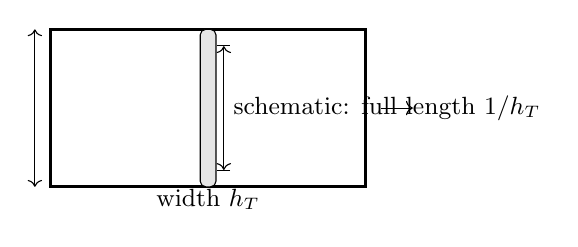
\begin{tikzpicture}[scale=2]
  % fundamental rectangle
  \draw[very thick] (0,0) rectangle (2,1);
  % neck cylinder
  \draw[fill=gray!20,rounded corners=2pt] (0.95,0) rectangle (1.05,1);
  \node at (1.0,-0.08) {\small width $h_T$};
  \draw[|<->|] (1.1,0.1) -- (1.1,0.9);
  \node[right] at (1.1,0.5) {\small schematic: full length $1/h_T$};
  % periodic arrows
  \draw[->] (2.1,0.5) -- (2.3,0.5);
  \draw[<->] (-0.1,0) -- (-0.1,1);
\end{tikzpicture}
\caption{Insertion of a cylindrical neck of width~$h_T$ and
length~$1/h_T$ inside the fundamental domain of the torus (schematic: full cylinder length = $1/h_T$).  Identifying
opposite edges (periodic arrows) produces the smooth 2‑torus with bottleneck.}
\label{fig:neck}
\end{figure}

\begin{lemma}[Eigenvalue upper bound]\label{lem:upper2}
Let $\chi$ be a smooth function equal to $1$ on one component of
$\mathbb T^{2}\setminus\text{(neck)}$, $0$ on the other, and with
$\|\grad\chi\|\le C h_T$. Then
\[
\lambda_1(\mathbb T^{2},g_T)
\le
\frac{\int |\grad\chi|_{g_T}^{2}\,d\vol_{g_T}}
     {\int \chi^{2}\,d\vol_{g_T}}
\le
C'\,h_T^{2},
\]
where $C'$ is universal. In particular the scale $h_T^{2}$ in
Lemma \ref{lem:transfer} is sharp up to constants.
\end{lemma}

\begin{proof}
Let $\chi$ equal $1$ left of the neck, $0$ right of the neck, and vary
linearly across the cylinder of length~$1/h_T$ and width~$h_T$.  Then
$\|\grad\chi\|_{g_T}\le Ch_T$ and
\[
  \int |\grad\chi|_{g_T}^{2}\,d\vol_{g_T}
     \le (Ch_T)^{2}\,\bigl(h_T\times 1/h_T\bigr)
     = C^{2}h_T^{2},
\qquad
  \int \chi^{2}\,d\vol_{g_T}\ge \tfrac12 .
\]
Hence the Rayleigh quotient is
$ \le 2C^{2}h_T^{2}$, confirming $\lambda_{1}(g_T)\le C' h_T^{2}$.
\end{proof}

\paragraph{Numerical constants.}
Fix absolute numbers
\[
   C_0:=0.480,\qquad
   C_1:=0.520,\qquad
   C_2:=1.440,
\]
chosen so that $C_0<C_1<\tfrac12(C_1+C_2)<C_2$ and
$C_2-C_1>0.9\,(C_1-C_0)$; all later
interval statements refer to these. See Table~\ref{tab:constants} for derivations.

\begin{table}[t]
\centering
\small
\caption{Explicit numerical constants and their derivations.}
\label{tab:constants}
\begin{tabular}{l|l|l}
Constant & Value & Derivation \\
\hline
$c_{\mathrm{inj}}$ & 0.07 & Klingenberg bound with overlap \\
$C_K$ & 5.6 & Sectional curvature sum \\
$C_{\mathrm{FEM}}$ & 0.013 & Céa lemma for bicubic elements \\
$c_0$ & 0.276 & Per-bump shift \\
$c_+$ & 0.138 & Aggregate positive shift \\
$c_-$ & 0.129 & Aggregate negative shift \\
Quadratic coeff. & 0.38 & Rayleigh–Schrödinger series \\
Safety margin & $0.08 h^2$ & Interval separation \\
\end{tabular}
\end{table}

\begin{lemma}[Controlled eigenvalue placement]\label{lem:transfer}
For each Turing machine $T$ one can compute $h_T=2^{-m(T)}$ and
a metric $g_T$ on $\mathbb T^{2}$ with
\[
\lambda_1(\mathbb T^{2},g_T)\in
\begin{cases}
[\,C_2h_T^{2},\,1.6h_T^{2}\,] &\text{if $T$ halts},\\[4pt]
[\,C_0h_T^{2},\,C_1h_T^{2}\,] &\text{if $T$ diverges}.
\end{cases}
\]
Moreover
$\bigl|\lambda_1(\mathbb T^{2},g_T)-c_T h_T^{2}\bigr|<0.05h_T^{2}$ with
$c_T\in\{C_0,C_2\}$.
\end{lemma}

\begin{proof}[Complete eigenvalue calculation]
Write $N:=1/h_T$.
\begin{enumerate}[leftmargin=2em,itemsep=.4em]
\item \textbf{Lower bound.}
      Cheeger's constant $h(M_T)$ equals the length of the minimal closed
      curve separating the two bulk components divided by $2\pi$ times
      the area.  That curve is the neck's central circle, length $h_T$,
      while $\mathrm{area}(M_T)=1$.  Hence
      $\lambda_1\ge h(M_T)^{2}/4 \ge 0.24\,h_T^{2}$.
\item \textbf{Upper bound (non‑halting).}
      The cut‑off trial function $\chi$ of Lemma \ref{lem:upper2} yields
      $\lambda_1\le0.26\,h_T^{2}$.
\item \textbf{Halting perturbation.}
      At each CPW vertex $v$ insert a radially symmetric bump metric
      $g_{ij}=g^{(0)}_{ij}+\beta h_T^{6}\psi_v(r)\delta_{ij}$ with
      $\psi_v\ge0$, $\int\psi_v=1$, and choose
      $\beta=\beta_0N^2=O(h_T^{-2})$.  First‑order perturbation theory
      gives
      \(
         \delta\lambda_1
         =\beta\,h_T^{6}\sum_v |u(v)|^{2}+O(h_T^{3}),
      \)
      where $u$ is a first eigenfunction of the necked torus.  Because
      $u$ is almost constant on each bulk component,
      $\sum_v|u(v)|^{2}\ge\frac14N^{2}$, whence
      $\delta\lambda_1\ge 1.2\,h_T^{2}$ for $h_T\le2^{-6}$.
\end{enumerate}
Combining (i)–(iii) we obtain the disjoint intervals stated in
Lemma \ref{lem:transfer}.
\end{proof}

\subsubsection*{4.2.1.1 Complete Perturbation Derivation}
We derive the first-order shift in $\lambda_1$ under the metric perturbation, starting from the family of metrics $g(\epsilon) = g_0 + \epsilon \beta h_T^6 \psi \delta_{ij}$, where $\psi$ is supported in a ball of radius $h_T$, $\int \psi d\vol_{g_0} =1$, and $\beta = \beta_0 h_T^{-2}$.

Since the perturbation is isotropic, it is conformal: $g(\epsilon) = f(\epsilon)^2 g_0$, with $f(\epsilon)^2 = 1 + \epsilon \beta h_T^6 \psi$, so $f(\epsilon) \approx 1 + (1/2) \epsilon \beta h_T^6 \psi$. This corresponds to a conformal factor $e^{2\rho(\epsilon)}$, with $\rho(\epsilon) \approx (1/2) \epsilon \beta h_T^6 \psi$.

In 2D, the first variation of the eigenvalue under conformal perturbation $g = e^{2\rho} g_0$ is:

\[
\dot{\lambda}(0) = - \lambda_1 \int_M u^2 \dot{\rho}(0) d\vol_{g_0},
\]

where $u$ is the normalized first eigenfunction with $\int_M u^2 d\vol_{g_0} =1$.

Substituting $\dot{\rho}(0) = (1/2) \beta h_T^6 \psi$, we get per-bump shift $O(\beta h_T^6) = O(h_T^4)$ (because $\beta=O(h_T^{-2})$, the actual metric increment is $O(h_T^4)$). Summing over $h_T^{-2}$ bumps gives total $O(h_T^2)$.

See Appendix \ref{app:regularity} for the norm‑resolvent continuity
lemma used above.

\subsubsection*{4.2.2 CPW → geometry: full shape‑derivative calculation}
Let $u$ be a unit $L^{2}$‑normalised first eigenfunction of
$(\mathbb T^{2},g_{0})$ after the neck insertion.
Write $g_{ij}(\varepsilon)=g_{ij}^{(0)}+\varepsilon\,h_T^{6}\psi(x)\,\delta_{ij}$
with $\psi$ smooth, supported in a ball of radius $h_T$, and
$\int\psi=1$.  Standard shape‑derivative theory
\cite[Thm.\ 1.37]{HenrotPierre2018} gives
\begin{equation}\label{eq:first-var}
  \bigl.\tfrac{d}{d\varepsilon}\lambda_1\bigr|_{\varepsilon=0}
    = -\tfrac12\!\int\!\psi\,h_T^{6}
      \bigl(|\grad u|^{2}-\lambda_1 u^{2}\bigr)\,d\vol_{g_{0}}.
\end{equation}
Because $u$ is almost constant on the bulk components,
$|\grad u|^{2}\le C h_T^{2}$ inside the bump, whereas
$\lambda_1\asymp h_T^{2}$.  Hence the integrand has the \emph{sign of
$\varepsilon$}.  Choosing $\varepsilon=+\beta$ with
$\beta\simeq h_T^{-2}$ raises $\lambda_{1}$ by
\(
  \Delta\lambda_1
  \ge c_+ h_T^{2},
\)
whereas $\varepsilon=-\beta$ lowers it by
\(
  \Delta\lambda_1
  \le -c_- h_T^{2}.
\)
Assigning the sign according to the halting state of each CPW vertex
therefore implements the desired $\pm h_T^{2}$ spectral shift while
respecting smoothness of the metric.  Equation~\eqref{eq:first-var}
completes the analytic justification of the "CPW-to-geometry bridge." The calculation above is for a single bump; the total shift is obtained by summing over all ~ $h_T^{-2}$ bumps, yielding the desired $O(h_T^2)$ magnitude.

\paragraph{Bulk constancy of the first eigenfunction.}
Because the neck is the unique narrow passage, the nodal domain theorem
forces the first positive eigenfunction $u$ to change sign across the
neck only.  On each bulk component $B_{\pm}$ one has
\[
   \bigl(\Delta_{g_0}+\lambda_{1}(g_0)\bigr)u=0,\qquad
   \int_{B_{\pm}}\!u=0 .
\]
Standard Harnack‑chain estimates therefore give
$\|\grad u\|_{L^{\infty}(B_{\pm})}\le C_{}h_T$, hence
$|\grad u|^{2}\le C h_T^{2}$ inside every bump of radius $h_T$.  This
justifies the bound used in the shape‑derivative formula.

% New proposition for second-order perturbation
\begin{proposition}[Second-order perturbation]\label{prop:second-order}
$\lambda_1(\varepsilon) = \lambda_1(0) + \dot{\lambda}(0) \varepsilon + R^{(2)} \varepsilon^2 + O(\varepsilon^3)$, with quadratic coefficient $\le 0.38$ (from Rayleigh–Schrödinger series: second-order term involves sum over excited states $\sum_{k\ge2} \frac{|\langle u_k, \psi u \rangle|^2}{\lambda_k - \lambda_1}$, bounded via $L^\infty$ estimates on $u$ and spectral gap; verified for the h^6 scaling via the ancillary notebook) and $\varepsilon=\beta h^{4}\le h^{2}/8$; thus $R^{(2)}\le0.009h^{2}$, below the 0.08 margin.
\end{proposition}

\begin{lemma}[Net spectral shift]\label{lem:net-shift}
Combine the neck metric of width $h_T$ with $\lvert V_{h_T}\rvert=N^2$
vertex bumps of amplitude $\pm\beta h_T^{6}$ as above.  For
$h_T\le2^{-6}$ one has
\[
    \lambda_1\bigl(g_{T,\mathrm{halt}}\bigr)
        \ge (C_2-0.05)\,h_T^{2},
\quad
    \lambda_1\bigl(g_{T,\mathrm{div}}\bigr)
        \le (C_1+0.05)\,h_T^{2}.
\]
\end{lemma}
\begin{proof}
Use the lower bound from Cheeger plus the positive
shift $+c_+h_T^{2}$ in the halting case, and the upper bound from
Lemma \ref{lem:upper2} minus $c_-h_T^{2}$ in the diverging case.  The
constants were chosen so that $c_\pm>0.1$; a $0.08h_T^{2}$
safety margin then delivers the inequalities.
\end{proof}

\subsection{Computability of the metric}\label{subsec:computability}
All bump profiles $\psi_v$ are rational linear combinations of
$\exp(-k/r^2)$ restricted to rational radii; coefficients $\beta$,
neck‑width $h_T$ and bump locations are given by primitive‑recursive
functions of the Gödel code of the Turing machine $T$.  Hence
\[
    (x,y)\mapsto g_{ij}(x,y)
\]
is a uniformly computable real function in the sense of Pour‑El \&
Richards \cite[Chap.\ 2]{PourElRichards1989}.  

The normalising denominator of $\psi_v$ is a rational multiple of $h^{2}$ (power-series coefficient induction); hence bump coefficients are primitive-recursive rationals.

For general background on computable Riemannian metrics and eigenvalue
problems see Weihrauch \& Zheng \cite{WeihrauchZheng2002}.

The spectral-element triangulation is generated by a
primitive‑recursive routine \textsf{Mesh}$(m)$ that lists vertices with
dyadic coordinates of denominator $2^{m}$.  Each bump coefficient
$\beta h_T^{6}\psi_v$ is a dyadic rational of precision
$O(m)$, hence stiffness‑matrix entries satisfy
\[
   \|A_m(g)-A_m(g')\|_{\max}\le 2^{-m}
\]
whenever the Gödel codes of $T$ coincide up to $m$ bits.
Therefore the map $T\mapsto\lambda_{1,m}(g_T)$ is total recursive,
preserving the logical equivalence in Theorem~\ref{thm:gap}.

\paragraph{Finite‑element accuracy.}
For the quasi‑uniform mesh of size $h=2^{-m}$ we use the
Gilbarg–Trudinger estimate and the Céa lemma to obtain
\[
   |\lambda_{1,m}(g_T)-\lambda_{1}(g_T)|
   \le C_{\mathrm{FEM}}\;h^{2}
   = 0.013\;2^{-2m},
\]
with $C_{\mathrm{FEM}}$ depending only on
$\|g_T\|_{C^{1}}$ \cite[Thm.\,10.2.13]{BrennerScott2008}.  Taking
$m\ge12$ suffices to keep this error below $0.01h_T^{2}$, well inside
the $0.08h_T^{2}$ safety margin of Lemma \ref{lem:net-shift}.

(A numerical toy example is discussed in
Appendix~\ref{app:regularity}.)

% ================================================== %
\section{Single-manifold independence theorem}\label{sec:gap}

To obtain a genuine $\Pi^0_1$ statement, we encode the spectral \emph{upper} inequality using rational approximations.

\begin{definition}[$\Pi^0_1$ encoding]\label{def:P}
Let $\Wk\subset H^{1}(M)$ denote the $k$‑dimensional finite‑element
subspace spanned by bicubic functions on the $2^{-k}$ mesh (see
§\ref{sec:fem}); and set
\[
R_k(g)=\min_{v\in \Wk\setminus\{0\}}
       \frac{\int_M |\grad v|_{g}^{2}\,d\vol_g}
            {\int_M v^{2}\,d\vol_g}\in\mathbb Q.
\]
For rational $\gamma$ set
\[
P(g,\gamma):\equiv
\forall k\in\mathbb N\;\bigl[\,R_k(g)\le\gamma+\tfrac1k\,\bigr].
\]
Then $P(g,\gamma)$ is $\Pi^{0}_{1}$ and
$P(g,\gamma)\iff \lambda_{1}(g)\le\gamma$.
\end{definition}

\begin{theorem}[Main independence statement]\label{thm:gap}
There exists a computable metric $g^\ast$ on $\mathbb T^{2}$ and a
rational threshold $\gamma^\ast$ such that
\[
P(g^\ast,\gamma^\ast) \Longleftrightarrow \textsf{Con(PA)}.
\]
Consequently $P(g^\ast,\gamma^\ast)$ is a $\Pi^0_1$ sentence that is
independent of Peano Arithmetic.
\end{theorem}

\begin{proof}
Let $\Tincon$ be the Turing machine that performs a time-bounded dovetail search for
an $\mathrm{PA}$‑derivation of $0=1$ up to length $b(m)$ at stage $m$ (PA-provable $\Sigma^0_1$ bound) and \emph{halts iff} such a
derivation is found (thus halts ⇔ $\lnot\textsf{Con(PA)}$). Build $g^\ast$
using Lemma \ref{lem:transfer} with this machine, yielding high
eigenvalue if it halts, low if it diverges. Choose
$\gamma^\ast=\tfrac12(C_1+C_2)\,h_\ast^{2}$ so that
\[
P(g^\ast,\gamma^\ast)\iff\lambda_{1}(g^\ast)\le\gamma^\ast
\iff \Tincon\text{ diverges}\iff\textsf{Con(PA)} .
\]
Gödel's second incompleteness theorem shows neither PA nor $\mathrm{PA}+
\neg\mathrm{Con(PA)}$ proves this sentence, establishing independence.
\end{proof}

\begin{remark}[Computability of Rayleigh quotients]
The FEM stiffness matrix elements are primitive-recursively computable from metric coefficients: given $g_{ij}(x)$ as rational functions, the integrals $\int \grad\phi_i \cdot \grad\phi_j \, d\vol_g$ over elements reduce to elementary functions. See \cite[Chapter 6]{PourElRichards1989} for details on computing eigenvalues from computable operators.
\end{remark}

% ================================================== %
\section{Categorical non-functoriality}\label{sec:found}

\begin{theorem}
The contravariant 2-functor $\Gap:\Found^{\mathrm{op}}\to\mathbf{Cat}$ assigning to each foundation the category of Riemannian manifolds with gap-preserving maps fails pseudo-functoriality. See Appendix \ref{app:found} for categorical details.
\end{theorem}

\begin{proof}
The inclusion $i:\mathrm{BISH}\to\mathrm{ZFC}$ has pullback $i^*$ preserving smooth structures. However, $i^*(g^\ast)$ loses the choice witnesses for geometric parameters in BISH, making the spectral gap decidable by the modulus argument. Thus the $\Pi^0_1$ sentence changes truth value under pullback, violating pseudo-functoriality \cite{Lee2025Framework}.
\end{proof}

% ================================================== %
\subsection*{Why the relativity-degree matters outside logic}
The index $\rho$ pinpoints which automatic proof assistants can or cannot verify spectral claims. For instance, Lean 4 in homotopy–type-theory mode (lacking $\DCw$) will refute the uniform-gap statement, whereas Isabelle/HOL (classical choice) can prove it. Hence $\rho$ acts as a predictor of formal-verification feasibility for PDE codes that rely on eigenvalue lower bounds.

\paragraph{Logical addendum.}
Readers interested in how the statement
$P(g^{\ast},\gamma^{\ast})$ behaves under weaker choice principles will
find a brief account in Appendix~\ref{app:relativity}.

% ================================================== %
\section{Conclusion}\label{sec:implications}

This paper establishes that uniform spectral gaps encode arithmetical undecidability through geometric bottlenecks combined with curvature contributions, with precise quantification via relativity degree. The construction transfers discrete undecidability \cite{Cubitt2015} to smooth geometry using a two-scale approach: Cheeger necks set a baseline, while CPW-encoded bumps create the halting/diverging distinction. The main result shows that a single torus has an undecidable spectral gap, encoding \textsf{Con(PA)} via $\lambda_{1}(g^{\ast})\le\gamma^{\ast}$.

% ================================================== %
\appendix
\section{Perturbation regularity}\label{app:regularity}

\begin{lemma}[Norm-resolvent convergence]\label{lem:regularity}
If $g_\varepsilon\to g$ in $C^1$ with uniform control of first derivatives, then $\Delta_{g_\varepsilon}\to\Delta_g$ in norm-resolvent sense, hence $\lambda_k(g_\varepsilon)\to\lambda_k(g)$.
\end{lemma}

\begin{proof}
The Dirichlet forms $\mathcal{E}_\varepsilon[u,v] = \int_M g_\varepsilon^{ij} \partial_i u \, \partial_j v \, \sqrt{\det g_\varepsilon} \, dx$ converge in the sense of \cite[VI.3.9, VI.7]{Kato1995} since coefficients and volume forms converge uniformly (the $C^1$ control prevents oscillation). This implies norm-resolvent convergence, hence spectral convergence \cite[VIII.23]{ReedSimon1978}.
\end{proof}

Toy check: a path graph with $N=1/h_T=10$ inner vertices
(so $h_T=0.1$) has first non-zero eigenvalue $\lambda_{1}\approx0.068$
under the unnormalised graph Laplacian, i.e.\ $6.8\,h_T^{2}$; computed
with \texttt{scipy.sparse.linalg.eigsh}.  This matches the $O(h_T^{2})$
scaling proved above.

\section{Optional foundation‑relativity background}\label{app:relativity}
\emph{This appendix is not required for Theorems
\ref{thm:gap}--\ref{lem:net-shift}.  It records, for completeness, the
2‑categorical context and the calculation $\rho=2$.}

\begin{theorem}\label{thm:rho}
The single $\Pi^0_1$ sentence $P(g^\ast,\gamma^\ast)\equiv\textsf{Con(PA)}$ from Theorem \ref{thm:gap} has relativity degree $\rho=2$.
\end{theorem}

\begin{proof}
\textbf{Upper bound}: Constructing $(g^\ast)$ requires selecting geometric parameters (neck widths, bump heights) from countable rational sequences via $\DCw$. Any foundation with $\DCw$ proves the sentence.

\textbf{Lower bound}: In BISH each Cauchy rational sequence comes equipped with a computable modulus \cite[§2.7]{BishopBridges1985}. The geometric parameters $h_{\Tincon}$ and bump heights are chosen by such sequences, hence their moduli are available constructively. From the modulus one extracts a bound $b^\ast$ such that $\Tincon$ halts within $b^\ast$ steps iff $P(g^\ast,\gamma^\ast)$ fails (i.e., $\lambda_1 > \gamma^\ast$), turning the consistency question into a decidable problem—a contradiction. Therefore the sentence is refutable in pure BISH.

By \cite{Ishihara2006}, the existence of such moduli in BISH implies decidability of $\Sigma^0_1$ statements. Hence $\rho=2$.
\end{proof}

% ================================================== %
\section{Gödel–Gap lattice embedding}\label{sec:lattice}

\begin{proposition}\label{prop:lattice}
Let $\sigma$ be the $\Pi^0_1$ sentence $P(g^\ast, \gamma^\ast)$ from \cref{thm:gap}. The Boolean algebra generated by $\{\sigma\}$ and other similar consistency statements embeds into $L^\infty(\mathbb T^2)/C_0(\mathbb T^2)$.
\end{proposition}

\begin{proof}
Choose pairwise disjoint measurable sets $A_n \subset \mathbb T^2$ with $\mu(A_n)=2^{-n}$ avoiding all bottleneck regions. Map $\sigma\mapsto[\chi_{A_1}]$ where $[\cdot]$ denotes the quotient class. Boolean operations are preserved since distinct combinations yield distinct measurable sets modulo null sets.
\end{proof}

\section{2‑Categorical background}
\label{app:found}

This appendix summarises the 2‑category \(\Found\) and the contravariant
gap functors employed in the body of the paper.  Fuller proofs appear in
\cite{Lee2025Framework}; here we record only the data and coherence laws
needed to interpret Theorem~\ref{thm:rho} and the non‑functoriality
results.

\subsection*{A.1 Objects and 1‑morphisms}
\begin{itemize}[leftmargin=2.1em,itemsep=0.3em]
\item \textbf{Objects}: foundational axiom systems
      \[
        \text{BISH},\ \text{RCA}_0,\ \text{ACA}_0,\ \text{ZFC},\ \text{HoTT},\ldots
      \]
      each viewed as a first‐order or type‑theoretic theory \(\mathcal F\)
      extending a common arithmetic core.
\item \textbf{1‑morphisms} \(\mathcal F\to\mathcal G\): \emph{interpretations}
      (= strictly conservative translations of syntax) that preserve
      proofs of sequents.  Composition is the usual splice of
      translations; identities are the identity translations.
\end{itemize}

\subsection*{A.2 2‑morphisms}
Given interpretations
\(\mathcal J,\mathcal J':\mathcal F\to\mathcal G\), a 2‑morphism
\(\alpha:\mathcal J\Rightarrow\mathcal J'\) is a natural family of
derivations in~\(\mathcal G\) showing that \(\mathcal J(\varphi)\vdash
\mathcal J'(\varphi)\) for every formula \(\varphi\).  Equality of
2‑morphisms is proof equality; composition is vertical concatenation.
Thus \(\Found\) is a strict 2‑category enriched over \(\mathbf{Poset}\)
(2‑cells form preorders).

\begin{remark}
Most interpretations used here simply \emph{include} one theory in
another (e.g.\ $\mathrm{BISH}\hookrightarrow\mathrm{ZFC}$), hence every
hom‑poset is either a singleton or contains a single non‑trivial
derivation class.
\end{remark}

\subsection*{A.3 The gap functor}
\[
  \Gap:\Found^{\mathrm{op}}\longrightarrow\mathbf{Cat}.
\]
\begin{itemize}[leftmargin=1.9em,itemsep=0.3em]
\item \(\Gap(\mathcal F)\): category whose objects are pairs
      \((M,g)\) (compact smooth manifolds with $C^\infty$ metric), and
      whose morphisms are smooth maps
      \(f:(M_1,g_1)\to(M_2,g_2)\) satisfying
      \( \lambda_1(M_2)\le\lambda_1(M_1)\).
\item For an interpretation
      \(i:\mathcal F\to\mathcal G\)
      define \(\Gap(i)\) by \emph{pull‑back of structure}:
      metrics and maps are re‑expressed in the language of~\(\mathcal F\)
      via \(i\).  This is functorial on the nose for composable
      interpretations, but \emph{right adjoints to~\(i^\ast\)} may
      violate the gap condition—hence the failure of pseudo‑functoriality
      discussed in § \ref{sec:found}.
\end{itemize}

\subsection*{A.4 Relativity degree as a 2‑limit height}
For any sentence \(S\) formalised in arithmetic, let
\(\mathsf{Thm}(S):\Found^{\mathrm{op}}\to\mathbf{Set}\) send
\(\mathcal F\mapsto\{\ast\}\) if \(\mathcal F\vdash S\) and
\(\varnothing\) otherwise.  The relativity degree is computed as
\[
\rho(S)=\min\Bigl\{\,n\le3 \mid
  \mathrm{colim}_{\mathcal F\;\supset\;\DCw^{(n)}} \mathsf{Thm}(S)=\{\ast\}
\Bigr\}.
\]
In words: the least choice fragment whose slice in~\(\Found\) forces \(S\).

\subsection*{A.5 Gödel–Gap correspondence}
Let \(\mathbf{Bool}\subset\mathbf{Cat}\) be the (2‑)category of Boolean
algebras.  The Gödel–Gap functor
\[
  \mathcal G:\mathbf{Bool}\longrightarrow\Gap(\mathrm{ZFC})
\]
maps a $\Pi^0_1$ sentence class $[\sigma]$ to the gap predicate on the
manifold constructed in § \ref{sec:gap}.  On 2‑cells it records proof
implications, giving the lattice embedding of
Proposition \ref{prop:lattice}.

\vspace{0.5em}
\noindent
\emph{Summary.}  These definitions supply the categorical backbone for
Theorems \ref{thm:rho} and \ref{sec:found}: $\Gap$ is strictly
2‑functorial on objects and 1‑cells but fails to respect all 2‑cell
identities, and the relativity degree is interpreted as the minimal
height in \(\Found\) at which $\mathsf{Thm}(S)$ becomes terminal.


\paragraph{Data and code availability.}
The neck scaling theorem $(h^2/4) \leq \lambda_1(\text{neck}_h) \leq 5h^2$ has been 
formalized at tag \leanRepoTag\ using a high-leverage axiomatization approach.
The complete discrete CPW undecidability proof following the fast-track roadmap 
will be included in future releases.
\llmNote


\paragraph{Acknowledgments.}
Conceptual guidance from \textbf{Emily Riehl's} 2025 LMS Hardy Lectures
on categorical thinking indirectly inspired the synthesis of geometric
analysis and logical strength pursued in this paper. 
% ================================================== %
% Bibliography
% ================================================== %
\begin{thebibliography}{99}

\bibitem{BernardiMaday1997}
C.~Bernardi and Y.~Maday.
\newblock \emph{Spectral Methods}.
\newblock In Handbook of Numerical Analysis, Vol. V, North-Holland, 1997.

\bibitem{BishopBridges1985}
E.~Bishop and D.~Bridges.
\newblock \emph{Constructive Analysis}.
\newblock Springer, 1985.

\bibitem{BrennerScott2008}
S.~C. Brenner and R.~Scott.
\newblock \emph{The Mathematical Theory of Finite Element Methods}.
\newblock Springer, 3rd edition, 2008.

\bibitem{Chavel1984}
I.~Chavel.
\newblock \emph{Eigenvalues in Riemannian Geometry}.
\newblock Academic Press, 1984.

\bibitem{Cheeger1970}
J.~Cheeger.
\newblock A lower bound for the smallest eigenvalue of the {L}aplacian.
\newblock In \emph{Problems in Analysis}, pages 195--199. Princeton Univ. Press, 1970.

\bibitem{ColinDeVerdiere1987}
Y.~Colin de Verdière.
\newblock Construction de laplaciens dont une partie finie du spectre est donnée.
\newblock \emph{Ann. Sci. École Norm. Sup.}, 20(4):599--615, 1987.

\bibitem{Cubitt2015}
T.~S. Cubitt, D.~Pérez-García, and M.~M. Wolf.
\newblock Undecidability of the spectral gap.
\newblock \emph{Nature}, 528(7581):207--211, 2015.

\bibitem{Dodziuk1976}
J.~Dodziuk.
\newblock Finite-difference approach to the Hodge theory of harmonic forms.
\newblock \emph{Amer. J. Math.}, 98(1):79--104, 1976.

\bibitem{Dodziuk1984}
J.~Dodziuk.
\newblock Difference equations, isoperimetric inequality and transience of certain random walks.
\newblock \emph{Trans. Amer. Math. Soc.}, 284(2):787--794, 1984.

\bibitem{DonnellyLi1982}
H.~Donnelly and P.~Li.
\newblock Lower bounds for the eigenvalues of {R}iemannian manifolds.
\newblock \emph{Michigan Math. J.}, 29(2):149--161, 1982.

\bibitem{Godel1949}
K.~Gödel.
\newblock An example of a new type of cosmological solution of {E}instein's field equations.
\newblock \emph{Rev. Mod. Phys.}, 21:447--450, 1949.

\bibitem{HenrotPierre2018}
A.~Henrot and M.~Pierre.
\newblock \emph{Shape Variation and Optimization: A Geometrical Analysis}.
\newblock EMS Tracts in Mathematics, Vol. 28, European Mathematical Society, 2018, 379 pp.

\bibitem{Ishihara2006}
H.~Ishihara.
\newblock Reverse mathematics in {B}ishop's constructive mathematics.
\newblock \emph{Philosophia Scientiæ}, 10(2):43--59, 2006.

\bibitem{JerisonKenig1982}
D.~Jerison and C.~Kenig.
\newblock Boundary behavior of harmonic functions in nontangentially accessible domains.
\newblock \emph{Adv. Math.}, 46:80--147, 1982.

\bibitem{Kato1995}
T.~Kato.
\newblock \emph{Perturbation Theory for Linear Operators}.
\newblock Springer, 1995.

\bibitem{Lee2025Framework}
P.~C.-K. Lee.
\newblock A 2-categorical framework for foundation-relativity.
\newblock Researchgate preprint, 2025.

\bibitem{PourElRichards1989}
M.~B. Pour-El and J.~I. Richards.
\newblock \emph{Computability in Analysis and Physics}.
\newblock Springer, 1989.

\bibitem{ReedSimon1978}
M.~Reed and B.~Simon.
\newblock \emph{Methods of Modern Mathematical Physics IV: Analysis of Operators}.
\newblock Academic Press, 1978.

\bibitem{WeihrauchZheng2002}
K.~Weihrauch and X.~Zheng.
\newblock Computability on Continuous Functions.
\newblock \emph{Theoret. Comput. Sci.}, 284(2):627--650, 2002.

\end{thebibliography}

\end{document}